\subsection{Linear Regression}
\subsubsection{GLM and MRSS}
\noindent
The convolution matrix we get from last section has five columns, which correspond to a column of 1's and 4 cond.txt files from our dataset, respectively. After we have created the convolution matrix, we use it as our design matrix and run the generalized linear regression on our image data. The dimension of our data is (64, 64, 34, 240). First, we reshape our data into 2 dimensional array, which has the shape of (64*64*34, 240). Then we pass our design matrix into the glm function to calculate the related beta hats. These 139624 beta hats we get from the regression correspond to the first three dimensions of our image data. For example, the first beta hat contains the information about the voxel (0,0,0). Then we turn the beta hats back into 4-dimensional shape and run the diagnostic functions on the 4-d beta hats. Based on the predictors, we can calculate the fitted values and then the residuals. We use the MRSS of the first three dimensions as a measurement of our regression. \newline

\begin{figure}[H]
    \centering
        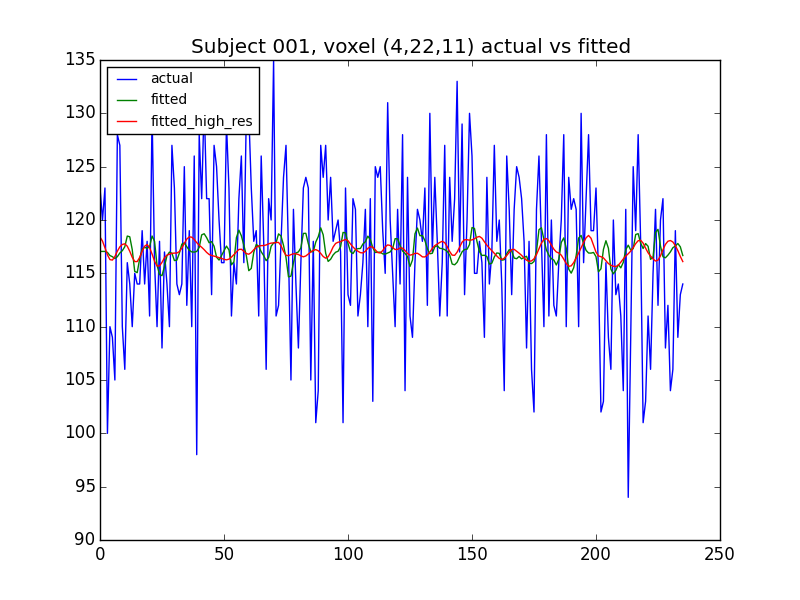
\includegraphics[scale=0.5]{../../plots/glm_fitted.png}
    \caption{fitted values for the linear regression}
\end{figure}


\noindent
After we tried the normal convolution, we also tried the high resolution convolution matrix. It turned out that the MRSS just reduced a little bit. Then we writing the smoothing function to implement the multidimensional Gaussian filter on our data. We repeat the same steps as what we have done in normal convolution on the smoothed data and the MRSS are reduced sharply. Therefore, we concluded that the smoothing method is a good pre-processing when we do the linear regression. \newline

\noindent
Below are the MRSS values for our subject 1, run 1: \newline
\begin{figure}[H]
    \centering
        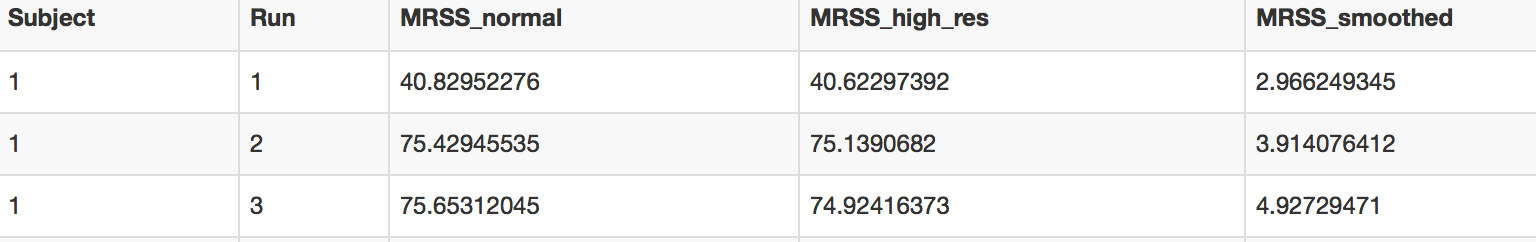
\includegraphics[scale=0.5]{../../plots/mrss_result001.png}
    \caption{MRSS for subject 1 run 1}
\end{figure}


\subsubsection{t-test and p-values}
\noindent
After getting the beta hats, we write the function for t-test, which will give us the corresponding t statistics and p values for our beta hats. Then we set our significant level to be $\alpha$ = 0.05; thus, if the beta has a p-value greater than or equal to 0.05, we will say that it is not significant; if the beta has a p-value smaller than 0.05, we will say that this voxel is activated. \newline
\noindent Therefore, we write a function called find\_activated\_voxel to change the voxel positions in the long list back to the 3-d voxel indices. We utilize the functions that we write for our homework to make transitions between them. After we get the positions of these significant voxels for our four predictors, we write them out into txt files. \newline


\subsubsection{Next Step}
\noindent
The affine attribute of the image contains the mapping from voxel coordinates to millimeters in the space of the image. Therefore, in our next step, we plan to get the mm coordinate for a particular voxel coordinate by applying this affine to our particular voxel coordinate, because the millmeter coordinate makes more sense if we want to do further analysis on the brain image. \newline
Besides, we haven't check the assumptions of regression. Therefore, we might check the normality and constant variance assumptions, but now we assume that these assumptions are satisfied since we have enough data. We also have the function to detect the outliers, so next time, we will get rid of the outliers before regression. \newline


